%------------------------------------------------------------------------------
\chapter{Active edge sensors}
\label{sec:appendixActiveEdge}
%------------------------------------------------------------------------------

TCAD simulation of active edge sensors using the process flow as
described in
\cref{sec:AdvacamProcessFlow}. \cref{fig:TCAD_dopingConcentration}
shows the concentration of the dopants. The nominal bias voltage is
also applied to the sensors and the region shown with a white line
corresponds to the depletion region.

\begin{figure}[htbp]
  \centering
  \begin{subfigure}[b]{0.5\linewidth}
    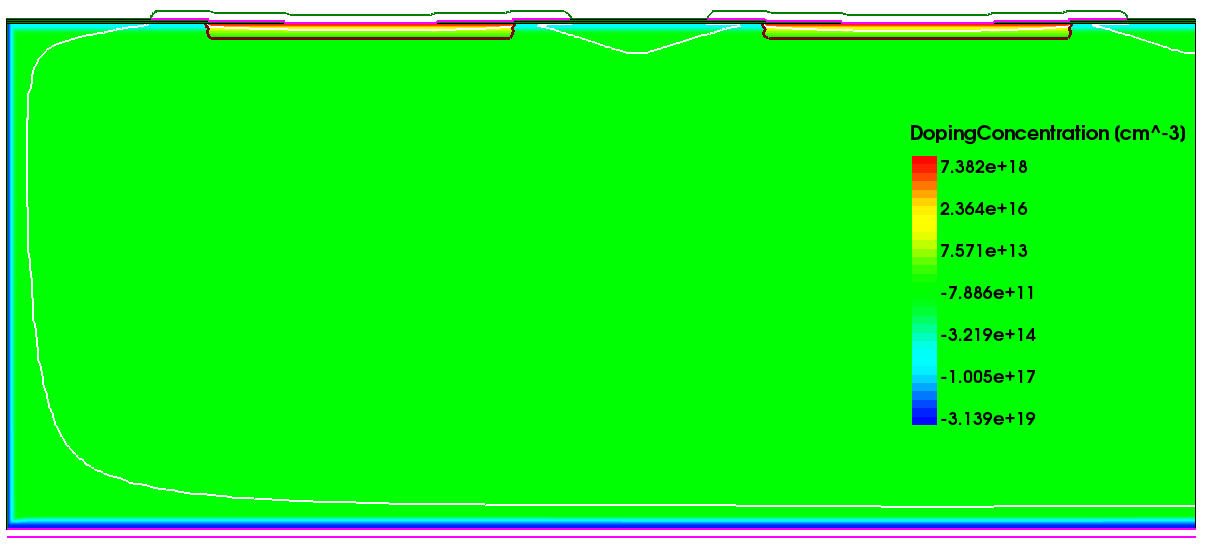
\includegraphics[width=\textwidth]{figures/TCAD/dopingConcentration_NoGR.png}
    \caption{20-NGR-50}
  \end{subfigure}\hfill
  \begin{subfigure}[b]{0.5\linewidth}
    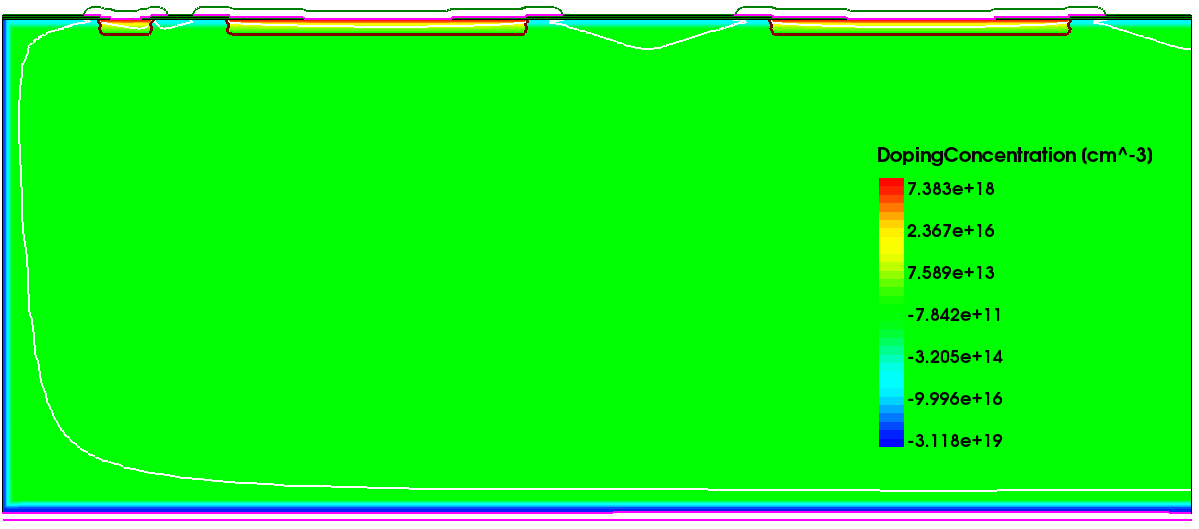
\includegraphics[width=\textwidth]{figures/TCAD/dopingConcentration_FloatGR.png}
    \caption{23-FGR-50}
  \end{subfigure} \\
  \begin{subfigure}[b]{0.5\linewidth}
    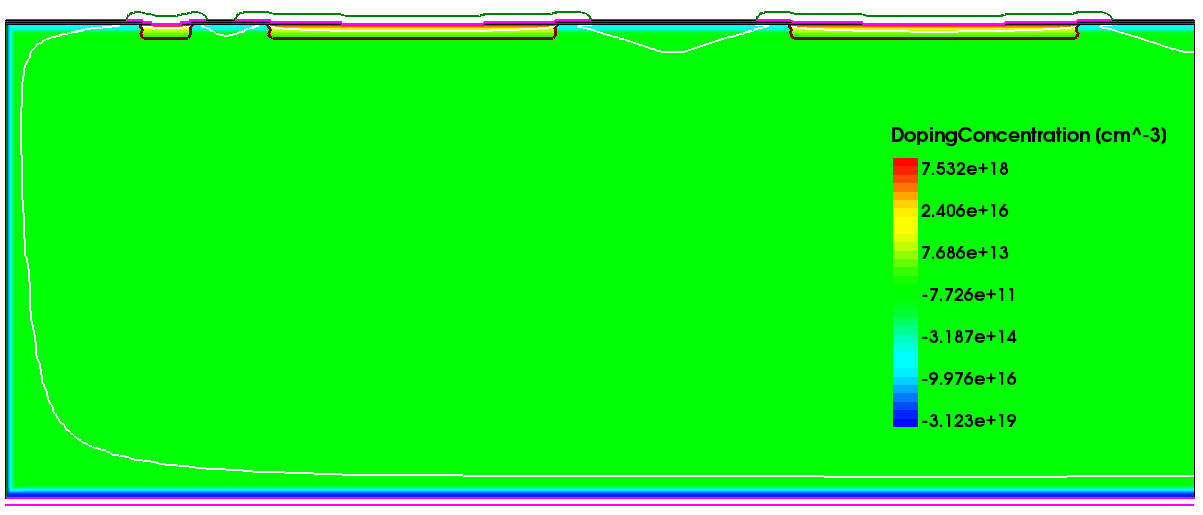
\includegraphics[width=\textwidth]{figures/TCAD/dopingConcentration_28_GNDGR.png}
    \caption{28-GNDGR-50}
  \end{subfigure}\hfill
  \begin{subfigure}[b]{0.5\linewidth}
    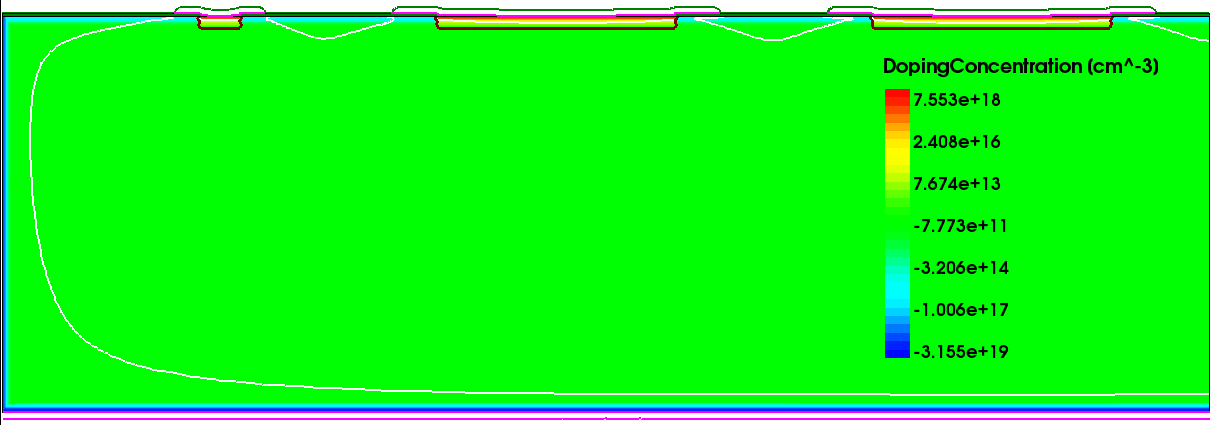
\includegraphics[width=\textwidth]{figures/TCAD/dopingConcentration_55_GNDGR.png}
    \caption{55-GNDGR-50}
  \end{subfigure} \\
  \begin{subfigure}[b]{0.5\linewidth}
    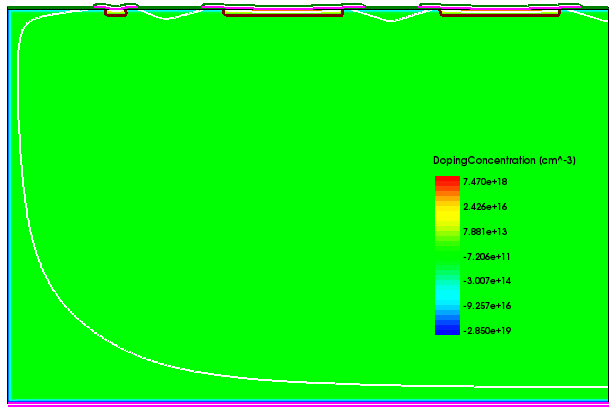
\includegraphics[width=\textwidth]{figures/TCAD/dopingConcentration_55_GNDGR_100.png}
    \caption{55-GNDGR-100}
  \end{subfigure}\hfill
  \begin{subfigure}[b]{0.5\linewidth}
    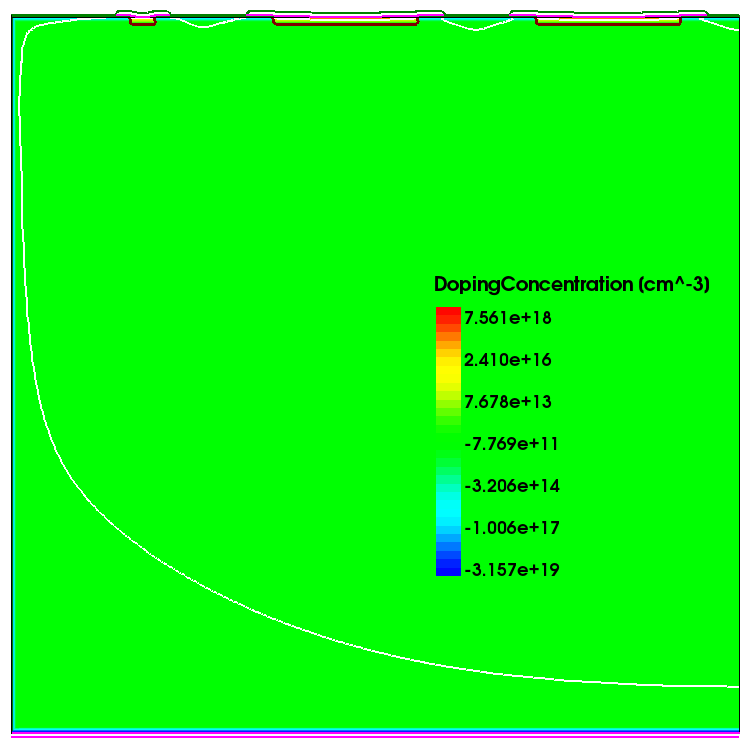
\includegraphics[width=\textwidth]{figures/TCAD/dopingConcentration_55_GNDGR_150.png}
    \caption{55-GNDGR-150}
  \end{subfigure}
  \caption{Doping concentration in TCAD simulations. The region shown
    with a white line is the depletion region.}
  \label{fig:TCAD_dopingConcentration}
\end{figure}
